\fancyhead[LE,RO]{\small\textbf{\textsf{MỤC 1.1}}\quad Bốn cách biểu diễn một hàm số\quad\textbf{15}}
\fancyhead[LO,RE]{}

\noindent
\begin{minipage}[t]{0.26\textwidth}
    \vspace{5.08cm}
    \begin{center}
        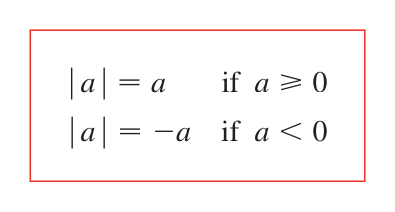
\includegraphics[width=0.95\linewidth]{images/p0050_fig1.png}
        \vspace{1mm}
        
        \textbf{\textsf{HÌNH 16}}
    \end{center}

    \vspace{1.8cm}
    \begin{center}
        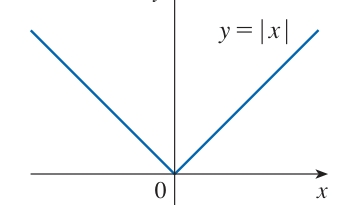
\includegraphics[width=0.95\linewidth]{images/p0050_fig2.png}
        \vspace{1mm}
        
        \textbf{\textsf{HÌNH 17}}
    \end{center}

    \vspace{1mm}
    \noindent\small Dạng phương trình đường thẳng qua một điểm với hệ số góc là $y - y_1 = m(x - x_1)$. Xem Phụ lục B.

    \vspace{3.44cm}
    \begin{center}
        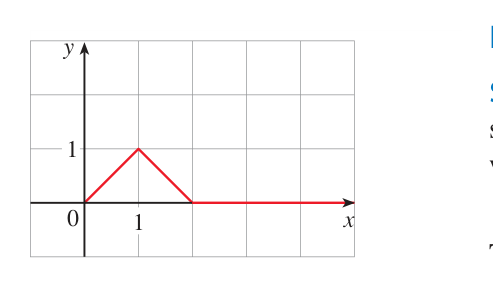
\includegraphics[width=0.95\linewidth]{images/p0050_fig3.png}
        \vspace{1mm}
        
        \textbf{\textsf{HÌNH 18}}
    \end{center}
\end{minipage}%
\hfill
\begin{minipage}[t]{0.71\textwidth}
Chẳng hạn,
\[
|3| = 3 \qquad |-3| = 3 \qquad |0| = 0 \qquad |\sqrt{2} - 1| = \sqrt{2} - 1 \qquad |3 - \pi| = \pi - 3
\]
Tổng quát, ta có
\begin{center}
\fcolorbox{stewartred}{white}{%
\parbox{0.48\textwidth}{%
\vspace{1.5mm}
\centering
$\begin{aligned}
|a| &= a \quad &&\text{nếu } a \ge 0\\[2mm]
|a| &= -a \quad &&\text{nếu } a < 0
\end{aligned}$
\vspace{1.5mm}
}%
}
\end{center}

\noindent (Hãy nhớ rằng nếu $a$ âm, thì $-a$ là số dương.)

\medskip
\noindent\textbf{\textsf{\color{stewartcyan}VÍ DỤ 8}}\quad Vẽ đồ thị của hàm giá trị tuyệt đối $f(x) = |x|$.

\noindent\textbf{\textsf{\color{stewartcyan}LỜI GIẢI}}\quad Từ phần thảo luận ở trên, ta biết rằng
\[
|x| = \begin{cases} 
x & \text{nếu } x \ge 0 \\ 
-x & \text{nếu } x < 0 
\end{cases}
\]
Sử dụng cùng phương pháp như trong Ví dụ 7, ta thấy rằng đồ thị của $f$ trùng với đường thẳng $y = x$ ở bên phải trục $y$ và trùng với đường thẳng $y = -x$ ở bên trái trục $y$ (xem Hình 16).\hfill{\color{stewartcyan}$\blacksquare$}

\medskip
\noindent\textbf{\textsf{\color{stewartcyan}VÍ DỤ 9}}\quad Tìm công thức cho hàm số $f$ có đồ thị trong Hình 17.

\noindent\textbf{\textsf{\color{stewartcyan}LỜI GIẢI}}\quad Đường thẳng đi qua $(0, 0)$ và $(1, 1)$ có hệ số góc $m = 1$ và tung độ gốc $b = 0$, do đó phương trình của nó là $y = x$. Vì vậy, đối với phần đồ thị của $f$ nối từ $(0, 0)$ đến $(1, 1)$, ta có
\[
f(x) = x \quad \text{nếu } 0 \le x \le 1
\]
Đường thẳng đi qua $(1, 1)$ và $(2, 0)$ có hệ số góc $m = -1$, do đó phương trình dạng điểm -- hệ số góc là
\[
y - 0 = (-1)(x - 2) \quad \text{hay} \quad y = 2 - x
\]
Nên ta có
\[
f(x) = 2 - x \quad \text{nếu } 1 < x \le 2
\]
Ta cũng thấy rằng đồ thị của $f$ trùng với trục $x$ khi $x > 2$. Kết hợp các thông tin này lại, ta có công thức ba phần sau đây cho hàm số $f$:
\[
f(x) = \begin{cases} 
x & \text{nếu } 0 \le x \le 1 \\ 
2 - x & \text{nếu } 1 < x \le 2 \\ 
0 & \text{nếu } x > 2 
\end{cases}
\tag*{\color{stewartcyan}$\blacksquare$}
\]

\noindent\textbf{\textsf{\color{stewartcyan}VÍ DỤ 10}}\quad Trong Ví dụ C ở đầu mục này, chúng ta đã xét chi phí $C(w)$ gửi một phong bì lớn có khối lượng $w$. Thực chất, đây là một hàm số xác định từng khúc bởi vì, từ Bảng 3, ta có
\[
C(w) = \begin{cases} 
1.00 & \text{nếu } 0 < w \le 1 \\ 
1.15 & \text{nếu } 1 < w \le 2 \\ 
1.30 & \text{nếu } 2 < w \le 3 \\ 
1.45 & \text{nếu } 3 < w \le 4 \\ 
\;\;\vdots & 
\end{cases}
\]
Đồ thị của hàm số này được cho trong Hình 18.\hfill{\color{stewartcyan}$\blacksquare$}
\end{minipage}